\subsection{Gesamtsystem}
Das Gesamtsystem wurde, wie bereits erwähnt, so günstig wie möglich aufgebaut. Wenn die einzelnen Komponenten bei den preiswertesten Lieferanten bezogen werden, dann kann das gesamte Gerät unter 150 CHF (exkl. Gehäuse) hergestellt werden. Die nachfolgende Tabelle (\tref{tKosten}) zeigt eine Auflistung der Kosten eines Gerätes. Zu den Kleinteilen zählen beispielsweise Schrauben oder Kabel.

\begin{table}[H]
\centering
    \begin{tabular}{p{5cm}l}
    \textbf{Komponente}                & \textbf{Preis}   \\
    NanoPi NEO                         & 10 CHF  \\
    Full HD Kamera                     & 50 CHF  \\
    Autobatterie                       & 50 CHF  \\ 
    WIFI-Adapter                       & 10 CHF  \\
    USB-Hub                            & 5 CHF   \\
    Spannungswandler                   & 10 CHF  \\
    Kleinteile						   & 15 CHF  \\ \hline
    \textbf{Gesamt}                    & \textbf{150 CHF} \\
    \end{tabular}
\caption{Kostenauflistung}
\label{tKosten}
\end{table}

Auf den folgenden Bildern wird das Gesamtsystem dargestellt. Dabei ist im ersten Bild ({\fref{bGesamtsystem}) das System in Grossansicht zu sehen, während im zweiten Bild ({\fref{bGesamtsystemH}) das System im Einsatz, hängend an einer Strassenlaterne, zu betrachten ist.

\begin{figure}[H]
  \centering
  
\includegraphics[height=0.4\textwidth]{Hardware/Gesamtsystem.jpg} 
  \caption{Gesamtsystem.}
  \label{bGesamtsystem}
\end{figure}

\begin{figure}[H]
  \centering
  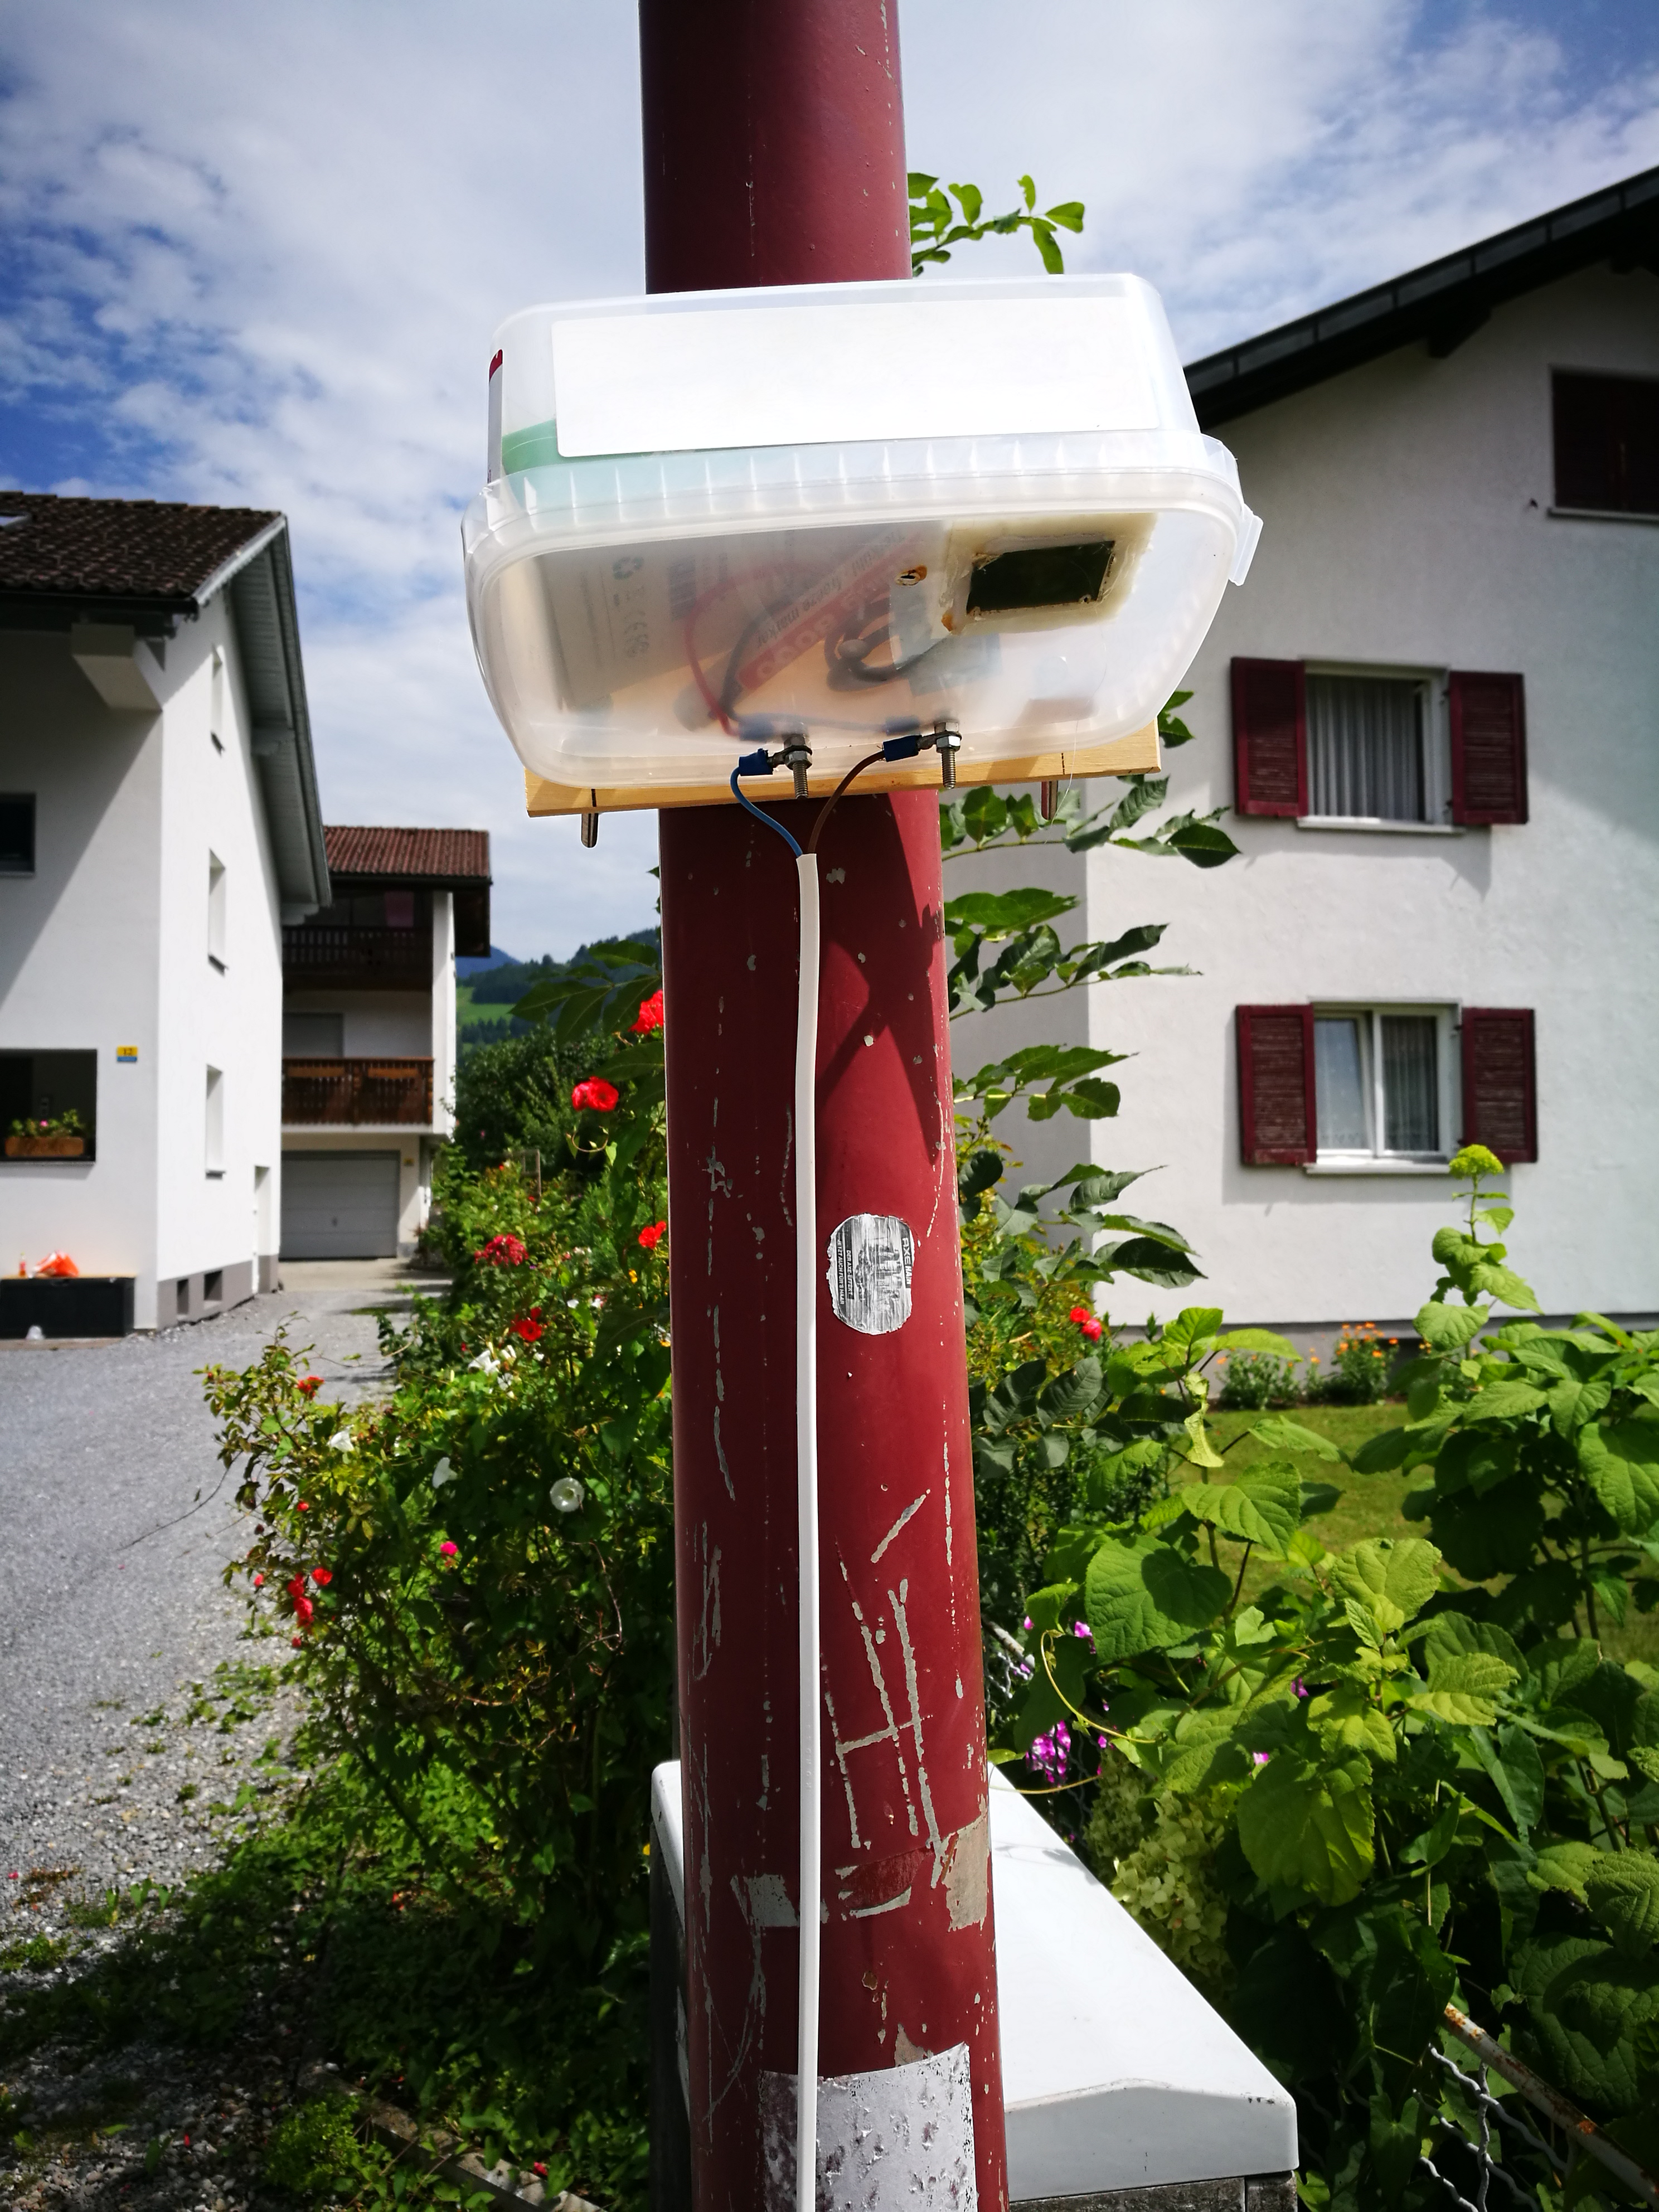
\includegraphics[height=0.99\textwidth]{Hardware/GesamtsystemH.jpg} 
  \caption{Einsatzfähiges Gesamtsystem.}
  \label{bGesamtsystemH}
\end{figure}